% !TEX program = xelatex
\documentclass[11pt,oneside]{report}

% ---------- Page geometry ----------
\usepackage[a4paper,margin=1in]{geometry}

% ---------- Fonts (XeLaTeX) ----------
\usepackage{fontspec}
\defaultfontfeatures{Ligatures=TeX}

% ---------- Math ----------
\usepackage{amsmath,amssymb,mathtools,bm}
\usepackage{bbm}

% ---------- Figures & graphics ----------
\usepackage{graphicx}
\usepackage[table]{xcolor}
\usepackage{tikz}
\usetikzlibrary{arrows.meta,positioning,calc,decorations.pathreplacing,fit}

% ---------- Tables ----------
\usepackage{booktabs}
\usepackage{tabularx}
\usepackage{longtable}
\usepackage{multirow}
\usepackage{array}

% ---------- Lists ----------
\usepackage{enumitem}
\setlist{itemsep=2pt, topsep=4pt}

% ---------- Captions ----------
\usepackage{caption}
\usepackage{subcaption}

% ---------- Hyperlinks ----------
\usepackage[hidelinks]{hyperref}
\usepackage[nameinlink,noabbrev]{cleveref}

% ---------- Bibliography ----------
\usepackage[numbers,sort&compress]{natbib}
\bibliographystyle{unsrtnat}

% ---------- Micro-typography ----------
\usepackage{microtype}

% ---------- Header/Footer ----------
\usepackage{fancyhdr}
\pagestyle{fancy}
\fancyhf{}
\fancyhead[L]{Flow Models \& Transformations in Physics}
\fancyhead[R]{\leftmark}
\fancyfoot[C]{\thepage}
\renewcommand{\headrulewidth}{0.4pt}
\setlength{\headheight}{26pt}

% ---------- Colors ----------
\definecolor{TableHeader}{RGB}{235,239,245}
\definecolor{RowA}{RGB}{250,250,252}
\definecolor{RowB}{RGB}{243,246,250}
\definecolor{BlueAccent}{RGB}{40,80,160}

% ---------- Useful macros ----------
\newcommand{\R}{\mathbb{R}}
\newcommand{\C}{\mathbb{C}}
\newcommand{\Z}{\mathbb{Z}}
\newcommand{\E}{\mathbb{E}}
\newcommand{\Var}{\mathrm{Var}}
\newcommand{\Cov}{\mathrm{Cov}}
\newcommand{\KL}{D_{\mathrm{KL}}}
\newcommand{\dd}{\mathrm{d}}
\newcommand{\tr}{\mathrm{tr}}
\newcommand{\diag}{\mathrm{diag}}
\newcommand{\sgn}{\mathrm{sgn}}

% Tight but readable paragraph spacing
\setlength{\parskip}{4pt}
\setlength{\parindent}{0pt}

% Better chapter title spacing
\usepackage{titlesec}
\titleformat{\chapter}[display]
  {\normalfont\bfseries\Huge\color{BlueAccent}}
  {\filleft\Large\chaptername\ \thechapter}
  {1ex}
  {\titlerule\vspace{1ex}\filright}
  [\vspace{1ex}\titlerule]

\begin{document}

% ---------- Title page ----------
\begin{titlepage}
\centering
\vspace*{2cm}
{\Huge\bfseries Flow Models and Flow Matching\\[0.35em]
\Large and\\[0.35em]
\Huge\bfseries Transformations and Ansatzes in Quantum Many-Body Physics\par}
\vspace{1.5cm}
{\Large Graduate-level report (XeLaTeX)\par}
\vspace{1.0cm}
{\large \today\par}
\vfill
\begin{minipage}{0.92\textwidth}
\textbf{Abstract.} 
\small
This report has two goals. 
\textbf{Part I} reviews the fundamentals of \emph{flow-based} generative modeling: the change-of-variables theorem, common architectural building blocks (coupling layers, autoregressive flows, invertible convolutions, and spline layers), and the continuous-time limit (continuous normalizing flows). We then explain \emph{flow matching} and \emph{conditional flow matching}, which train continuous-time flows without differentiating through ODE solvers. We also discuss modeling \emph{discrete} data with flows, including dequantization, integer/discrete coupling, and surjective constructions, with an emphasis on pros/cons and practical trade-offs.

\textbf{Part II} surveys a wide set of \emph{transformations} and \emph{variational ans"atze} used across quantum many-body physics, especially in condensed matter and quantum information. We provide a table that organizes these methods by goal (constraints, correlations, mappings, diagonalization, decoupling, dualities, and modern variational families), and then derive each method in detail: Gutzwiller projection, Jastrow correlators, Laughlin and composite-fermion constructions, Jordan--Wigner and Bravyi--Kitaev mappings, Bogoliubov transformations, matchgates/fermionic Gaussian states, Hubbard--Stratonovich decouplings, Schrieffer--Wolff canonical transformations, Kramers--Wannier duality, bosonization, spin-boson mappings (Holstein--Primakoff and Schwinger bosons), tensor-network ans"atze, coupled-cluster methods, and neural-network quantum states.
\end{minipage}
\vfill
\end{titlepage}

% ---------- Front matter ----------
\pagenumbering{roman}
\setcounter{tocdepth}{2}
\tableofcontents
\listoffigures
\listoftables

\cleardoublepage
\pagenumbering{arabic}

% ============================================================
% PART I
% ============================================================
\part{Flow Models and Flow Matching}

\chapter{Preliminaries: Change of Variables and Flow Objectives}
\section{Change of variables and exact likelihoods}
A \emph{normalizing flow} constructs a complicated probability density by pushing forward a simple base density through an \emph{invertible} mapping. Let $\mathbf{z}\in\R^d$ be a latent variable with known density $p_Z(\mathbf{z})$ (e.g. standard Gaussian), and let $f_\theta:\R^d\to\R^d$ be a diffeomorphism (invertible, differentiable, differentiable inverse). The data variable is
\begin{equation}
\mathbf{x} = f_\theta(\mathbf{z}),\qquad \mathbf{z} = f_\theta^{-1}(\mathbf{x}).
\end{equation}
Then the induced density on $\mathbf{x}$ is given by the change-of-variables theorem:
\begin{equation}
 p_X(\mathbf{x}) = p_Z\big(f_\theta^{-1}(\mathbf{x})\big)\,\left|\det \frac{\partial f_\theta^{-1}(\mathbf{x})}{\partial \mathbf{x}}\right|.
\label{eq:cov}
\end{equation}
Equivalently, in log form,
\begin{equation}
\log p_X(\mathbf{x}) = \log p_Z(\mathbf{z}) - \log\left|\det \frac{\partial f_\theta(\mathbf{z})}{\partial \mathbf{z}}\right|\Bigg|_{\mathbf{z}=f_\theta^{-1}(\mathbf{x})}.
\label{eq:loglik}
\end{equation}
A dataset $\{\mathbf{x}^{(n)}\}_{n=1}^N$ can thus be trained by exact maximum likelihood (minimizing negative log-likelihood). The two computational bottlenecks in \eqref{eq:loglik} are:
\begin{enumerate}
\item efficient evaluation of $f_\theta^{-1}(\mathbf{x})$ (the inverse map), and
\item efficient evaluation of the log-determinant of the Jacobian.
\end{enumerate}
Flow architectures are therefore designed to make these operations tractable.

\section{A taxonomy of flow layers}
Flow layers can be organized by how they achieve tractability:
\begin{itemize}
\item \textbf{Coupling layers} (NICE/RealNVP/Glow): exact inverse and triangular Jacobian; expressive via stacking and permutation.
\item \textbf{Autoregressive flows} (MAF/IAF): triangular Jacobian but sequential structure; either sampling or density is fast, not both.
\item \textbf{Invertible linear transforms}: permutations, invertible $1\times1$ convolutions, orthogonal/PLU parameterizations.
\item \textbf{Elementwise monotone transforms}: splines, rational-quadratic couplings.
\item \textbf{Continuous-time flows} (CNFs): define $\dot{\mathbf{x}}=v_\theta(t,\mathbf{x})$; log-density changes by divergence.
\end{itemize}
\Cref{tab:flowlayers} summarizes common layer types.

\begin{table}[h!]
\centering
\rowcolors{2}{RowA}{RowB}
\begin{tabularx}{\textwidth}{>{\raggedright\arraybackslash}p{3.2cm} X p{3.3cm}}
\rowcolor{TableHeader}
\textbf{Layer family} & \textbf{Key idea} & \textbf{Cost characteristics}\\
\toprule
Coupling (additive/affine) & Split variables $\mathbf{x}=(\mathbf{x}_a,\mathbf{x}_b)$; leave $a$ unchanged; transform $b$ using a NN conditioned on $a$. Jacobian is triangular. & Fast inverse and log-det; requires multiple layers for mixing.\\
Autoregressive (MAF/IAF) & Each dimension transformed conditioned on previous ones. Jacobian triangular by construction. & One direction is sequential (slow).\\
Invertible linear (permute, 1x1 conv) & Mix channels/dimensions between nonlinear layers to improve expressivity. & Log-det often cheap (e.g. $\log|\det W|$).\\
Spline/monotone elementwise & Replace affine maps by monotone splines (e.g. rational-quadratic). & More expressive, still tractable inverse and log-det.\\
Residual / ODE (CNF) & Define continuous dynamics $\dot{\mathbf{x}}=v(t,\mathbf{x})$; log-density evolves via divergence. & Training/sampling require ODE solves unless using flow matching.\\
\bottomrule
\end{tabularx}
\caption{A pragmatic taxonomy of flow layers and their computational trade-offs.}
\label{tab:flowlayers}
\end{table}

\section{Visual intuition: a coupling layer}
\Cref{fig:coupling} illustrates the architecture of an affine coupling layer.

\begin{figure}[h!]
\centering
\begin{tikzpicture}[font=\small, node distance=9mm, >=Latex]
\node[draw, rounded corners, minimum width=1.9cm, minimum height=0.85cm] (x) {$\mathbf{x}$};
\node[draw, rounded corners, right=20mm of x, minimum width=2.2cm, minimum height=0.85cm] (split) {split};
\node[draw, rounded corners, right=20mm of split, minimum width=2.5cm, minimum height=0.85cm] (nn) {NN $\to (s,t)$};
\node[draw, rounded corners, below=10mm of nn, minimum width=2.5cm, minimum height=0.85cm] (aff) {$\mathbf{x}_b\odot e^{s}+t$};
\node[draw, rounded corners, right=22mm of nn, minimum width=1.9cm, minimum height=0.85cm] (ya) {$\mathbf{y}_a=\mathbf{x}_a$};
\node[draw, rounded corners, right=22mm of aff, minimum width=1.9cm, minimum height=0.85cm] (yb) {$\mathbf{y}_b$};
\node[draw, rounded corners, right=16mm of ya, minimum width=1.9cm, minimum height=0.85cm] (y) {$\mathbf{y}$};

\draw[->] (x) -- (split);
\draw[->] (split) -- node[above]{$\mathbf{x}_a$} (nn);
\draw[->] (split) |- node[left]{$\mathbf{x}_b$} (aff);
\draw[->] (nn) -- (ya);
\draw[->] (nn) -- (aff);
\draw[->] (aff) -- (yb);
\draw[->] (ya) -- (y);
\draw[->] (yb) -- (y);

\node[below=2mm of split] {$\mathbf{x}=(\mathbf{x}_a,\mathbf{x}_b)$};
\node[below=2mm of y] {$\mathbf{y}=(\mathbf{y}_a,\mathbf{y}_b)$};
\end{tikzpicture}
\caption{Affine coupling layer: $\mathbf{y}_a=\mathbf{x}_a$, $\mathbf{y}_b=\mathbf{x}_b\odot\exp s(\mathbf{x}_a)+t(\mathbf{x}_a)$. Inverse is immediate: $\mathbf{x}_a=\mathbf{y}_a$, $\mathbf{x}_b=(\mathbf{y}_b-t(\mathbf{y}_a))\odot\exp[-s(\mathbf{y}_a)]$.}
\label{fig:coupling}
\end{figure}

\chapter{Discrete-time Flows: RealNVP, Glow, Autoregressive and Spline Flows}
\section{Coupling layers: NICE and RealNVP}
Coupling layers originate from NICE \citep{dinh2015nice} and RealNVP \citep{dinh2017realnvp}. The simplest form is \emph{additive coupling}:
\begin{equation}
\mathbf{y}_a = \mathbf{x}_a,\qquad \mathbf{y}_b = \mathbf{x}_b + t_\theta(\mathbf{x}_a).
\end{equation}
The Jacobian is triangular with unit diagonal, hence \emph{volume preserving} (log-det $=0$). RealNVP generalizes to an \emph{affine} coupling
\begin{equation}
\mathbf{y}_a = \mathbf{x}_a,\qquad \mathbf{y}_b = \mathbf{x}_b\odot \exp(s_\theta(\mathbf{x}_a)) + t_\theta(\mathbf{x}_a),
\label{eq:affinecoupling}
\end{equation}
so that
\begin{equation}
\log\left|\det \frac{\partial \mathbf{y}}{\partial \mathbf{x}}\right| = \sum_i s_{\theta,i}(\mathbf{x}_a).
\end{equation}
Why is this expressive? A single coupling layer only changes half the variables, so we stack many such layers and alternate the split (or apply permutations) so that every dimension is eventually modified. In image models, the split is often a channel-wise split, and the NN is a convolutional network.

\section{Multi-scale architectures and squeezing}
Flow-based image models commonly use a \emph{multi-scale} architecture: after some transformations, part of the variables are ``factored out'' as latent variables, reducing the dimensionality of subsequent layers. This improves efficiency and encourages the model to represent coarse features early and fine details later. In RealNVP, a ``squeeze'' operation reshapes spatial dimensions into channels (e.g. $H\times W\times C \mapsto (H/2)\times (W/2)\times 4C$), enabling channel-wise coupling to capture local pixel correlations.

\section{Glow and invertible 1\texorpdfstring{$\times$}{x}1 convolutions}
Glow \citep{kingma2018glow} improves RealNVP by introducing:
\begin{enumerate}
\item \textbf{ActNorm}: an affine per-channel normalization initialized from data (like batch norm but deterministic at test time), and
\item \textbf{Invertible $1\times1$ convolutions}: a learned linear mixing of channels per spatial location, parameterized by an invertible matrix $W\in\R^{C\times C}$.
\end{enumerate}
For an invertible $1\times1$ convolution applied to each spatial location, the log-determinant is $HW\log|\det W|$. Glow parameterizes $W$ via an LU decomposition so that $\log|\det W|$ is cheap to compute.

\section{Autoregressive flows: MAF and IAF}
Autoregressive flows use the factorization $p(\mathbf{x})=\prod_i p(x_i\mid x_{<i})$ but in an invertible transform. A typical autoregressive transform is
\begin{equation}
 y_i = \mu_i(\mathbf{x}_{<i}) + \sigma_i(\mathbf{x}_{<i})\,x_i,
\end{equation}
which yields a triangular Jacobian. Masked Autoregressive Flow (MAF) \citep{papamakarios2017maf} makes density evaluation fast (because all $y_i$ can be computed in parallel), but inversion/sampling is sequential. Inverse Autoregressive Flow (IAF) \citep{kingma2016iaf} swaps the roles to make sampling fast but density slow. This illustrates a general trade-off: autoregressive structure enforces triangular Jacobians but introduces sequential dependence in at least one direction.

\section{Spline flows and monotone transforms}
Affine couplings can be replaced by more expressive monotone elementwise transforms. Neural spline flows \citep{durkan2019nsf} use rational-quadratic splines whose parameters are predicted by a NN. Because the spline is monotone on each interval, it is invertible; both the inverse and the log-derivative can be computed analytically. In practice, spline couplings improve likelihood and sample quality at similar computational cost.

\section{Residual flows and invertible ResNets}
Another design is to use residual connections while enforcing invertibility. A residual flow has the form
\begin{equation}
\mathbf{y} = \mathbf{x} + g_\theta(\mathbf{x}),
\end{equation}
which is invertible if $g_\theta$ is a contraction (e.g. Lipschitz constant $<1$). Then the Jacobian determinant can be approximated via power-series of $\log\det(I+J_g)$ and trace estimators. Residual flows connect to continuous-time flows and ODE interpretations.

\chapter{Continuous Normalizing Flows and Flow Matching}
\section{Continuous-time limit and the log-density ODE}
A continuous normalizing flow (CNF) defines dynamics
\begin{equation}
\frac{\dd \mathbf{x}(t)}{\dd t} = v_\theta(t,\mathbf{x}(t)),\qquad t\in[0,1],
\label{eq:cnf}
\end{equation}
with $\mathbf{x}(0)\sim p_0$ and $\mathbf{x}(1)$ as the generated sample. The instantaneous change of log-density along trajectories is
\begin{equation}
\frac{\dd}{\dd t}\log p_t(\mathbf{x}(t)) = -\nabla\cdot v_\theta(t,\mathbf{x}(t)).
\label{eq:logpODE}
\end{equation}
Derivation sketch: write the continuity equation $\partial_t p_t + \nabla\cdot(p_t v)=0$, then take the material derivative along a trajectory and use $\frac{\dd}{\dd t}p_t(\mathbf{x}(t))=\partial_t p_t + v\cdot\nabla p_t$.

Likelihood evaluation thus requires integrating \eqref{eq:cnf} and \eqref{eq:logpODE}. CNFs such as FFJORD \citep{grathwohl2019ffjord} use Hutchinson trace estimators to approximate $\nabla\cdot v$ without forming the full Jacobian, reducing cost from $O(d^2)$ to roughly $O(d)$ per evaluation.

\section{Why flow matching?}
Training CNFs by maximum likelihood can be expensive because it involves repeated ODE solves and backpropagation through the solver (often via the adjoint method). \textbf{Flow Matching} (FM) \citep{lipman2023flowmatching} reframes training as \emph{supervised vector-field regression} that does not require solving the generative ODE during training.

The starting point is a \emph{probability path} $\{p_t\}_{t\in[0,1]}$ connecting $p_0$ (noise) to $p_1$ (data). Any sufficiently smooth path admits a velocity field $u^*(t,\mathbf{x})$ satisfying the continuity equation
\begin{equation}
\partial_t p_t(\mathbf{x}) + \nabla\cdot\big(p_t(\mathbf{x})u^*(t,\mathbf{x})\big)=0.
\end{equation}
If we learn $u_\theta\approx u^*$, then integrating $\dot{\mathbf{x}}=u_\theta(t,\mathbf{x})$ transports $p_0$ approximately into $p_1$.

\section{Flow matching objective}
FM chooses a tractable way to sample from $p_t$ and to compute (or sample) the target velocity. A particularly useful instantiation is \textbf{conditional flow matching} (CFM): sample an endpoint $\mathbf{x}_1\sim q_1$ from the data distribution, sample $\mathbf{x}_0\sim p_0$ from the base distribution, and define a conditional interpolation $\mathbf{x}_t=\phi_t(\mathbf{x}_0\mid \mathbf{x}_1)$. A simple choice is linear interpolation
\begin{equation}
\mathbf{x}_t = (1-t)\mathbf{x}_0 + t\mathbf{x}_1,\qquad \dot{\mathbf{x}}_t = \mathbf{x}_1-\mathbf{x}_0.
\label{eq:linearpath}
\end{equation}
Then we can train $u_\theta$ via mean-square regression
\begin{equation}
\mathcal{L}_{\mathrm{FM}}(\theta)=\E_{t\sim\mathrm{Unif}[0,1]}\E_{\mathbf{x}_0\sim p_0,\,\mathbf{x}_1\sim q_1}\big\|u_\theta(t,\mathbf{x}_t) - (\mathbf{x}_1-\mathbf{x}_0)\big\|^2.
\label{eq:fmobj}
\end{equation}
More sophisticated paths (e.g. diffusion-type paths or optimal-transport paths) can reduce stiffness and improve sample quality. Lipman \emph{et al.} show that FM can match or exceed diffusion models on image generation tasks while enabling ODE-based sampling and likelihood evaluation \citep{lipman2023flowmatching,albergo2023multisample}.

\section{Relation to diffusion models and score matching}
Diffusion models define a forward noising process that maps data $\mathbf{x}_1\sim q$ to noise $\mathbf{x}_0\sim p_0$ by an SDE, and train a score network to reverse it \citep{sohl2015diffusion,ho2020ddpm,song2021scorebased}. Flow matching can be viewed as learning a deterministic vector field whose trajectories approximate a chosen probability path. When the path is chosen as the marginal of an SDE, the FM objective becomes closely related to denoising-score matching, but with a regression target that is often more numerically stable.

\section{A minimal algorithmic template}
\begin{enumerate}
\item Sample $\mathbf{x}_1\sim q_1$ (data), $\mathbf{x}_0\sim p_0$ (noise), and $t\sim\mathrm{Unif}[0,1]$.
\item Compute $\mathbf{x}_t = \phi_t(\mathbf{x}_0\mid \mathbf{x}_1)$ (e.g. \eqref{eq:linearpath}).
\item Regress $u_\theta(t,\mathbf{x}_t)$ to the known target velocity (e.g. $\mathbf{x}_1-\mathbf{x}_0$).
\item After training, sample by solving $\dot{\mathbf{x}}=u_\theta(t,\mathbf{x})$ from $t=0$ to $1$ with initial $\mathbf{x}(0)\sim p_0$.
\end{enumerate}
Flow matching thus replaces expensive ``simulate-then-differentiate'' loops with ``sample-and-regress'' training.

\chapter{Discrete Data and Discrete Flows}
\section{Why discrete data is subtle}
The change-of-variables formula \eqref{eq:cov} relies on a Lebesgue density and a Jacobian determinant. For purely discrete variables $x\in\{0,1\}^N$ or $x\in\{0,\dots,255\}^N$, probability is defined with respect to counting measure, so a deterministic bijection $f$ merely permutes probability mass. If the base distribution is factorized or uniform, a bijection alone cannot create arbitrary target probabilities.

This observation motivates three broad strategies:
\begin{enumerate}
\item \textbf{Dequantization}: embed discrete data in continuous space by adding noise.
\item \textbf{Stochastic / surjective flows}: allow non-invertible maps augmented with auxiliary noise.
\item \textbf{Truly discrete flows}: define invertible transformations in a discrete algebra (e.g. modular arithmetic) and combine with expressive base distributions.
\end{enumerate}

\section{Dequantization for images}
For integer pixel data $\mathbf{x}\in\{0,\dots,255\}^D$, define a continuous variable
\begin{equation}
\mathbf{y} = \mathbf{x} + \mathbf{u},\qquad \mathbf{u}\sim \mathrm{Unif}([0,1)^D).
\end{equation}
Train a continuous density model $p_\theta(\mathbf{y})$; this yields a lower bound on the discrete likelihood of $\mathbf{x}$ by integrating $p_\theta$ over the unit hypercube around $\mathbf{x}$. Flow++ \citep{ho2019flowpp} introduced \emph{variational dequantization}: instead of uniform noise, learn a conditional noise distribution $q_\phi(\mathbf{u}\mid \mathbf{x})$ using an auxiliary flow, tightening the bound and improving likelihood.

\section{Discrete flows: invertible transforms on finite alphabets}
Discrete normalizing flows aim to model $p(\mathbf{x})$ exactly without dequantization. A common design is a discrete coupling layer for $K$-ary variables $x\in\{0,\dots,K-1\}^D$ using modular arithmetic:
\begin{equation}
\mathbf{y}_a = \mathbf{x}_a,\qquad \mathbf{y}_b = (\mathbf{x}_b + t_\theta(\mathbf{x}_a))\bmod K.
\end{equation}
This is invertible because subtraction mod $K$ is well-defined. Such constructions appear in integer discrete flows and discrete flows for sequences \citep{tran2019discreteflows,hoogeboom2019integer}. The main challenge is expressiveness: because there is no Jacobian term, the model must rely on an expressive \emph{base} distribution and deep compositions.

\section{Binary data: flows on \texorpdfstring{$\{0,1\}^N$}{\{0,1\}^N}}
For binary vectors, modular addition is XOR. A binary coupling can be written as
\begin{equation}
\mathbf{y}_a=\mathbf{x}_a,\qquad \mathbf{y}_b = \mathbf{x}_b \oplus t_\theta(\mathbf{x}_a),
\end{equation}
where $t_\theta(\mathbf{x}_a)\in\{0,1\}^{|b|}$. This is invertible since XOR is its own inverse. However, XOR couplings alone are limited because they cannot change Hamming weight patterns smoothly; expressive modeling often requires adding latent noise (surjective flows) or hybridizing with autoregressive components.

\section{Surjective flows and latent-variable constructions}
Surjective/augmented flows relax bijectivity by introducing auxiliary variables $\mathbf{u}$ so that the map $(\mathbf{x},\mathbf{u})\mapsto \mathbf{z}$ is bijective, but $\mathbf{x}\mapsto \mathbf{z}$ is not. This allows true changes in probability mass. SurVAE flows \citep{nielsen2020survae} unify VAEs and flows by combining surjective and stochastic layers with tractable likelihood bounds. In practice, surjective flows can model discrete data more flexibly than purely bijective discrete flows.

\section{Pros and cons summary}
\begin{table}[h!]
\centering
\rowcolors{2}{RowA}{RowB}
\begin{tabularx}{\textwidth}{>{\raggedright\arraybackslash}p{3.1cm} X X}
\rowcolor{TableHeader}
\textbf{Approach} & \textbf{Pros} & \textbf{Cons}\\
\toprule
Dequantization & Leverages mature continuous-flow toolkit; scalable to images; good likelihoods. & Not an exact discrete model; choice of dequantization distribution affects bound.\\
Pure discrete bijective flows & Exact likelihood on discrete space; no Jacobian computations. & Expressiveness limited unless base distribution is rich; design/inference can be hard at large alphabet size.\\
Surjective / stochastic flows & Can change mass and model complex discreteness; unifies flows and VAEs. & Usually gives bounds not exact likelihood; additional variance and design complexity.\\
\bottomrule
\end{tabularx}
\caption{High-level trade-offs in modeling discrete data with flow-based methods.}
\label{tab:discreteproscons}
\end{table}

\chapter{Flows in Physics: Symplectic and Equivariant Constraints (Brief)}
Flows have also been adapted to respect physical structure. In Hamiltonian mechanics, canonical transformations preserve the symplectic form; Li \emph{et al.} proposed \emph{symplectic flows} as neural canonical transformations \citep{li2019neuralct}. In molecular modeling, equivariant flows enforce $E(3)$ symmetry (rotations/translations) to model configurations. These ideas echo a recurring theme in physics: powerful transformations are those that preserve the relevant geometry (symplectic, gauge, or symmetry constraints).

% ============================================================
% PART II
% ============================================================
\part{Transformations and Ansatzes in Quantum Many-Body Physics}

\chapter{Overview and Summary Table}
\section{Why transformations and ans"atze matter}
Quantum many-body Hilbert spaces grow exponentially. Two broad strategies help:
\begin{enumerate}
\item \textbf{Transformations}: rewrite the Hamiltonian or degrees of freedom into a form where the physics is clearer or the problem is solvable (exactly or approximately). Examples include mappings between spins and fermions (Jordan--Wigner), auxiliary-field decouplings (Hubbard--Stratonovich), and canonical transformations (Schrieffer--Wolff).
\item \textbf{Variational ans"atze}: propose a family of wavefunctions with manageable complexity that captures key correlations (Gutzwiller, Jastrow, Laughlin) or obeys entanglement constraints (tensor networks).
\end{enumerate}
These tools are ubiquitous: from integrable 1D models to quantum Hall physics, from superconductivity to quantum simulation on qubits.

\section{A roadmap table}
\rowcolors{2}{RowA}{RowB}
\begin{longtable}{p{3.8cm} p{3.4cm} p{6.9cm}}
\caption{Survey table of transformations and ans"atze covered in Part II. The ``Type'' column labels the dominant role: mapping/transform (T) or variational ansatz (A).}\label{tab:bigtable}\\
\rowcolor{TableHeader}\textbf{Method} & \textbf{Type} & \textbf{Core idea and typical use}\\
\toprule
\endfirsthead
\rowcolor{TableHeader}\textbf{Method} & \textbf{Type} & \textbf{Core idea and typical use}\\
\toprule
\endhead
\bottomrule
\endfoot
Gutzwiller projector & A & Enforce strong local constraints (e.g. no double occupancy) by projecting a mean-field wavefunction. Useful for Hubbard/t-J and spin liquids.\\
Jastrow correlator / Feenberg & A & Multiply a reference state by $\exp(\sum_{i<j}u(r_{ij}))$ to incorporate pair correlations and cusp conditions.\\
Laughlin wavefunction & A & Holomorphic Jastrow polynomial in LLL producing incompressible FQH liquids; leads to fractional charge/anyons.\\
Composite fermions / flux attachment & T/A & Singular gauge transformation attaching $2p$ flux quanta (Chern--Simons); maps FQH fractions to integer QH of composite fermions.\\
Jordan--Wigner mapping & T & Map 1D spins to fermions via a nonlocal parity string; solves Ising/XY chains and encodes fermions on qubits.\\
Bravyi--Kitaev mapping & T & Alternative fermion-to-qubit transform with shorter Pauli strings (logarithmic locality) for quantum simulation.\\
Bogoliubov (BdG) transformation & T & Canonical linear transform mixing $c$ and $c^\dagger$ to diagonalize quadratic Hamiltonians (BCS, superfluids).\\
Matchgates and fermionic Gaussian states & T & Quadratic fermionic unitaries correspond to orthogonal transforms of Majoranas; matchgate circuits are classically simulable.\\
Hubbard--Stratonovich decoupling & T & Rewrite quartic interactions as integrals over auxiliary fields; basis for mean-field and determinantal QMC.\\
Schrieffer--Wolff canonical transform & T & Unitary perturbative elimination of high-energy subspace; yields effective low-energy Hamiltonians (t-J, Kondo).\\
Particle--hole transformation & T & Exchange particles and holes; reveals symmetries (e.g. bipartite Hubbard) and simplifies pairing problems.\\
Kramers--Wannier duality & T & Map Ising order operators to disorder operators; exposes self-dual criticality and dual phases.\\
Bosonization & T & Map 1D fermions/spins to bosonic fields; yields Luttinger liquids, universal exponents.\\
Holstein--Primakoff spin-wave expansion & T/A & Represent spins as bosons about an ordered state; derive magnon dispersions and $1/S$ corrections.\\
Schwinger bosons / partons & T/A & Express spins in terms of fractionalized bosons/fermions with gauge constraints; build spin-liquid ans"atze.\\
Tensor networks (MPS/PEPS/MERA) & A & Variational families structured by entanglement; MPS for 1D gapped systems, PEPS for 2D, MERA for criticality.\\
Coupled cluster and unitary coupled cluster & A & Exponential ansatz $e^T|\Phi\rangle$ (or $e^{T-T^\dagger}$) for correlated ground states; central in quantum chemistry and many-body theory.\\
Neural-network quantum states & A & Parameterize amplitudes by neural nets (RBM, autoregressive, equivariant); flexible variational ansatz for correlated phases.\\
\end{longtable}

\chapter{Gutzwiller Projection and Jastrow Correlators}
\section{Gutzwiller projector: definition and physical meaning}
Consider the Hubbard model
\begin{equation}
H = -t\sum_{\langle ij\rangle,\sigma}(c_{i\sigma}^\dagger c_{j\sigma}+\mathrm{h.c.}) + U\sum_i n_{i\uparrow}n_{i\downarrow}.
\end{equation}
At large $U/t$, double occupancy is energetically costly. A variational way to encode this is the \textbf{Gutzwiller wavefunction} \citep{gutzwiller1963}:
\begin{equation}
|\Psi_G\rangle = P_G(g)\,|\Psi_0\rangle,\qquad P_G(g)=\prod_i \big[1-(1-g)\,n_{i\uparrow}n_{i\downarrow}\big],
\label{eq:gutz}
\end{equation}
where $|\Psi_0\rangle$ is typically a Slater determinant or BCS state and $g\in[0,1]$ tunes the weight of doubly occupied sites. The limit $g=0$ enforces the constraint $n_{i\uparrow}n_{i\downarrow}=0$ on every site, appropriate for the $U\to\infty$ Mott regime.

\subsection{Projecting a Slater determinant: from metal to Mott}
If $|\Psi_0\rangle$ is a Fermi sea, then $|\Psi_G\rangle$ is a highly correlated state. The projection entangles the degrees of freedom because it correlates occupations on each site. One can see this by writing the amplitude of a configuration $|\{n_{i\uparrow},n_{i\downarrow}\}\rangle$:
\begin{equation}
\Psi_G(\{n\}) = g^{D(\{n\})}\,\Psi_0(\{n\}),\qquad D(\{n\})=\sum_i n_{i\uparrow}n_{i\downarrow}.
\end{equation}
Thus the projector is a simple scalar weight $g^D$ in the occupation basis.

\subsection{Gutzwiller approximation: renormalization factors}
A commonly used analytical approximation replaces expectation values in $|\Psi_G\rangle$ by renormalizing hopping and exchange processes. For example, a hopping process $c_{i\sigma}^\dagger c_{j\sigma}$ is suppressed because it can create double occupancy. In the Gutzwiller approximation, one estimates
\begin{equation}
\langle c_{i\sigma}^\dagger c_{j\sigma}\rangle_G \approx g_t\,\langle c_{i\sigma}^\dagger c_{j\sigma}\rangle_0,
\end{equation}
with $g_t$ a doping-dependent factor. For the $t$--$J$ model at hole doping $\delta$ (electron density $1-\delta$) one obtains
\begin{equation}
 g_t = \frac{2\delta}{1+\delta},\qquad g_J = \frac{4}{(1+\delta)^2},
\end{equation}
where $g_J$ renormalizes superexchange terms $\mathbf{S}_i\cdot\mathbf{S}_j$. These formulas can be derived by simple counting of allowed local configurations under the projection (probability that a hop is allowed in the projected ensemble divided by that in the unprojected ensemble). While uncontrolled, the approximation is qualitatively useful and underlies renormalized mean-field theories of cuprates.

\section{Jastrow correlators: from cusp conditions to long-range order}
A \textbf{Jastrow} wavefunction multiplies a reference state by an explicit correlator \citep{jastrow1955,foulkes2001qmc}:
\begin{equation}
|\Psi_J\rangle = \exp\Big(\frac{1}{2}\sum_{i\neq j} u_{ij}\,\hat{O}_i\hat{O}_j\Big)\,|\Phi\rangle.
\label{eq:jastrowop}
\end{equation}
In continuum electron systems, $\hat{O}_i$ is often the density at position $\mathbf{r}_i$ and $u_{ij}=u(|\mathbf{r}_i-\mathbf{r}_j|)$. For lattice models, common choices are density-density Jastrow factors $\exp(\sum_{i<j} v_{ij} n_i n_j)$ or spin Jastrow factors.

\subsection{Deriving the electron-electron cusp condition}
For Coulomb-interacting electrons, the wavefunction must satisfy a cusp condition as two electrons approach. Consider two electrons with relative coordinate $r$ and reduced mass $\mu=m/2$. Near $r=0$, the Schr"odinger equation in relative coordinates is dominated by
\begin{equation}
\left(-\frac{1}{2\mu}\frac{\dd^2}{\dd r^2} + \frac{e^2}{r}\right)\psi(r) \approx E\psi(r).
\end{equation}
Neglecting $E$ and higher terms, one finds that $\psi'(0^+)/\psi(0)=\mu e^2$ (up to spin-dependent factors). A Jastrow factor with $u(r)\sim a r$ at small $r$ can enforce this cusp by making $\psi(r)\sim e^{-u(r)/2}\approx 1-(a/2)r+\cdots$.

\subsection{Long-range Jastrow and Luttinger liquids}
In 1D, long-range Jastrow correlators can generate Luttinger-liquid exponents. For example, a wavefunction with
\begin{equation}
 u_{ij}\propto -K\log\left|\sin\frac{\pi(i-j)}{L}\right|
\end{equation}
produces power-law correlations characteristic of a Luttinger parameter $K$. This foreshadows the deep connections between Jastrow forms, bosonization, and conformal field theory wavefunctions.

\chapter{Quantum Hall Ans"atze: Laughlin and Composite Fermions}
\section{Lowest Landau level and holomorphic structure}
For a charged particle in a perpendicular magnetic field, the kinetic energy forms Landau levels separated by $\hbar\omega_c$. In the lowest Landau level (LLL), wavefunctions in symmetric gauge take the form
\begin{equation}
\psi(z,\bar z)=f(z)\,\exp\Big(-\frac{|z|^2}{4\ell_B^2}\Big),\qquad z=x+iy,
\end{equation}
where $f(z)$ is holomorphic. Many-body fermionic states in the LLL are therefore antisymmetric holomorphic polynomials times the Gaussian.

\section{Laughlin wavefunction and filling fraction}
The Laughlin ansatz at filling $\nu=1/m$ (odd $m$ for fermions) is \citep{laughlin1983}:
\begin{equation}
\Psi_m(z_1,\dots,z_N)=\prod_{i<j}(z_i-z_j)^m\,\exp\Big(-\sum_k\frac{|z_k|^2}{4\ell_B^2}\Big).
\label{eq:laughlin}
\end{equation}
The factor $(z_i-z_j)^m$ ensures an $m$-th order zero when particles coincide, suppressing close encounters and lowering Coulomb energy. On the sphere, the relation between number of flux quanta $N_\phi$ and particle number is $N_\phi=m(N-1)$; thus $\nu\approx N/N_\phi\to 1/m$ for large $N$.

\subsection{Quasiholes and fractional charge}
A quasihole at position $\eta$ is created by
\begin{equation}
\Psi_{\mathrm{qh}}(\eta)=\prod_i(z_i-\eta)\,\Psi_m.
\end{equation}
By adiabatically inserting one flux quantum, one produces a deficit of charge $e/m$. The Berry phase for braiding two quasiholes yields an anyonic statistical phase $\theta=\pi/m$.

\subsection{Plasma analogy (sketch)}
$|\Psi_m|^2$ can be interpreted as the Boltzmann weight of a 2D one-component plasma at inverse temperature $\beta=2m$. This analogy explains screening and incompressibility, and provides intuition for fractionalization.

\section{Flux attachment and composite fermions}
A powerful transformation for FQH physics is \textbf{flux attachment}: attach $2p$ flux quanta to each electron via a singular gauge transformation, mapping interacting electrons at filling $\nu$ to \emph{composite fermions} at an effective filling. In first-quantized form, define
\begin{equation}
\Psi_{\mathrm{CF}} = \prod_{i<j}\left(\frac{z_i-z_j}{|z_i-z_j|}\right)^{2p}\,\Psi_{e},
\end{equation}
which multiplies the wavefunction by a phase that depends on particle positions and changes the effective statistics of the attached flux.

Field-theoretically, this corresponds to introducing a Chern--Simons gauge field $a_\mu$ with constraint
\begin{equation}
\frac{1}{2\pi}\,\epsilon^{ij}\partial_i a_j = 2p\,\rho,
\end{equation}
so that the CS magnetic field is proportional to density. In mean-field, $\rho$ is replaced by its average so composite fermions see an effective magnetic field
\begin{equation}
 B^* = B - 2p\,\rho\,\phi_0,
\end{equation}
with $\phi_0=h/e$. If composite fermions fill $n$ effective Landau levels, one obtains Jain fractions
\begin{equation}
\nu = \frac{n}{2pn\pm 1}.
\end{equation}
This transformation provides a unifying picture of many observed FQH states \citep{jain1989cf,zhang1989cs}.

\chapter{Spin--Fermion and Fermion--Qubit Mappings}
\section{Jordan--Wigner transformation in 1D}
On a 1D chain, define fermion operators by
\begin{equation}
 c_j = \left(\prod_{k<j}\sigma_k^z\right)\,\sigma_j^-,\qquad c_j^\dagger = \left(\prod_{k<j}\sigma_k^z\right)\,\sigma_j^+.
\label{eq:jw}
\end{equation}
The nonlocal string ensures fermionic anticommutation: for $i<j$, $\{c_i,c_j\}=0$ because the string in $c_j$ contains $\sigma_i^z$ which anticommutes with $\sigma_i^-$. One also finds $\sigma_j^z=1-2c_j^\dagger c_j$.

\subsection{Example: transverse-field Ising to Kitaev chain}
The 1D transverse-field Ising model
\begin{equation}
H=-J\sum_j \sigma_j^x\sigma_{j+1}^x - h\sum_j \sigma_j^z
\end{equation}
maps under Jordan--Wigner to a quadratic fermion Hamiltonian with pairing terms. In Majorana variables $\gamma_{j,1}=c_j+c_j^\dagger$, $\gamma_{j,2}=i(c_j^\dagger-c_j)$, one obtains the Kitaev chain form, revealing Majorana edge modes in the ordered phase.

\section{Bravyi--Kitaev transformation}
Jordan--Wigner strings have length $O(N)$, which is costly for quantum simulation. The Bravyi--Kitaev (BK) transformation \citep{bravyi2002fermionic,seeley2012bk} balances locality of parity and occupancy information, reducing typical Pauli-string lengths to $O(\log N)$. BK can be understood as encoding each fermionic mode's occupation and parity in a binary tree structure. The explicit mapping can be described via three sets (update, parity, flip sets) defining which qubits store which parity bits. While more complex, BK often reduces circuit depth for chemistry Hamiltonians.

\chapter{Quadratic Fermions: Bogoliubov and Matchgates}
\section{General quadratic Hamiltonians and Nambu space}
A general fermionic quadratic Hamiltonian can be written as
\begin{equation}
H = \sum_{ij} c_i^\dagger A_{ij} c_j + \frac{1}{2}\sum_{ij}\left(c_i^\dagger B_{ij} c_j^\dagger + \mathrm{h.c.}\right),
\end{equation}
where $A$ is Hermitian and $B$ is antisymmetric. Define the Nambu spinor $\Psi=(c_1,\dots,c_N,c_1^\dagger,\dots,c_N^\dagger)^T$. Then
\begin{equation}
H = \frac{1}{2}\Psi^\dagger\begin{pmatrix}A & B\\ -B^* & -A^T\end{pmatrix}\Psi + \mathrm{const}.
\label{eq:bdg}
\end{equation}
Diagonalization amounts to finding a linear transformation $\Psi = W\Gamma$ that preserves canonical anticommutation. Such $W$ are elements of a Bogoliubov group (a subgroup of $U(2N)$ with particle-hole constraints).

\section{Bogoliubov transformation and BCS}
For each momentum pair $(k,-k)$ in BCS mean-field, the Hamiltonian reduces to a $2\times2$ Bogoliubov--de Gennes block. The canonical transform
\begin{equation}
\gamma_k = u_k c_k + v_k c_{-k}^\dagger,
\end{equation}
with $|u_k|^2+|v_k|^2=1$, diagonalizes the block, yielding quasiparticle energies $E_k=\sqrt{\xi_k^2+|\Delta|^2}$ \citep{bcs1957,bogoliubov1958}.

\section{Majorana representation and Gaussian states}
Define Majorana operators
\begin{equation}
\gamma_{2j-1}=c_j+c_j^\dagger,\qquad \gamma_{2j}=i(c_j^\dagger-c_j),
\end{equation}
which satisfy $\{\gamma_a,\gamma_b\}=2\delta_{ab}$. Quadratic Hamiltonians generate orthogonal transformations on Majoranas: a Gaussian unitary $U=\exp(-\frac{i}{4}\gamma^T K\gamma)$ acts as
\begin{equation}
U^\dagger\gamma U = R\gamma,\qquad R\in SO(2N).
\end{equation}
Gaussian states are fully characterized by the covariance matrix $\Gamma_{ab}=\frac{i}{2}\langle[\gamma_a,\gamma_b]\rangle$.

\section{Matchgates as fermionic Gaussian circuits}
A \textbf{matchgate} is a two-qubit gate that preserves fermionic Gaussianity under the Jordan--Wigner mapping. Valiant showed that nearest-neighbor matchgate circuits are classically simulable \citep{valiant2002matchgates}; Jozsa and Miyake clarified the connection to fermionic linear optics \citep{jozsa2010matchgates}. The simulation proceeds by updating the covariance matrix under each local orthogonal transformation.

\chapter{Auxiliary-Field Transformations: Hubbard--Stratonovich}
\section{Gaussian integral identity}
The Hubbard--Stratonovich (HS) transformation uses the Gaussian identity
\begin{equation}
\exp\left(\frac{\lambda}{2}O^2\right)=\frac{1}{\sqrt{2\pi}}\int_{-\infty}^{\infty}\dd \phi\,\exp\left(-\frac{\phi^2}{2}+\sqrt{\lambda}\,\phi\,O\right),\qquad \lambda>0.
\label{eq:hs}
\end{equation}
This linearizes a quadratic operator $O^2$ at the cost of integrating over an auxiliary field $\phi$.

\section{Decoupling the Hubbard interaction}
In determinantal QMC, one Trotter-decomposes $e^{-\beta H}$ into time slices and decouples the on-site interaction $U n_{\uparrow}n_{\downarrow}$ via an HS field. A standard discrete HS (Hirsch) writes
\begin{equation}
 e^{-\Delta\tau U\left(n_{\uparrow}-\frac12\right)\left(n_{\downarrow}-\frac12\right)} = \frac12\sum_{s=\pm 1} e^{\alpha s(n_{\uparrow}-n_{\downarrow})},\qquad \cosh\alpha = e^{\Delta\tau U/2}.
\end{equation}
Then fermions become quadratic for fixed $\{s_{i,\tau}\}$, allowing integration and yielding a determinant weight \citep{blankenbecler1981dqmc,hirsch1985dqmc}.

\section{Mean-field as saddle point}
The same HS transformation underlies mean-field theory: in a path integral, one introduces a field $\phi(\tau)$ and approximates the integral by its saddle point $\phi\approx\phi_0$. The saddle-point condition yields the mean-field self-consistency equation (e.g. BCS gap equation when decoupling in the pairing channel).

\chapter{Canonical Transformations: Schrieffer--Wolff and Particle--Hole}
\section{Schrieffer--Wolff: general idea}
Suppose $H=H_0+V$, where $H_0$ has a large gap separating low-energy (L) and high-energy (H) subspaces, and $V$ weakly couples them. The Schrieffer--Wolff (SW) transformation seeks a unitary $e^{S}$ (with $S$ anti-Hermitian) such that
\begin{equation}
H_{\mathrm{eff}} = e^{S}He^{-S}
\end{equation}
has no matrix elements between L and H to a desired order. Expanding,
\begin{equation}
H_{\mathrm{eff}} = H + [S,H] + \frac12[S,[S,H]]+\cdots.
\end{equation}
Choosing $S$ so that $V+[S,H_0]=0$ (off-diagonal part) eliminates coupling at first order, producing an effective Hamiltonian in L at second order.

\section{Application: Hubbard to t--J}
At large $U$, take $H_0=U\sum_i n_{i\uparrow}n_{i\downarrow}$ and $V$ the hopping. Eliminating virtual double-occupancy processes yields the t--J model
\begin{equation}
H_{tJ} = -t\sum_{\langle ij\rangle,\sigma}\tilde c_{i\sigma}^\dagger \tilde c_{j\sigma} + J\sum_{\langle ij\rangle}\left(\mathbf{S}_i\cdot\mathbf{S}_j-\frac14 n_in_j\right),\qquad J=\frac{4t^2}{U},
\end{equation}
where $\tilde c$ act in the no-double-occupancy subspace. The exchange term arises from a second-order process where an electron hops to form a doubly occupied intermediate state then hops back, producing an effective antiferromagnetic coupling.

\section{Particle--hole transformation on bipartite lattices}
On a bipartite lattice, the Hubbard model has a particle--hole symmetry at half filling. Define
\begin{equation}
 c_{i\downarrow}\mapsto (-1)^i c_{i\downarrow}^\dagger,
\end{equation}
where $(-1)^i$ is $+1$ on one sublattice and $-1$ on the other. This maps repulsive $U$ to attractive $U$ and relates antiferromagnetism to $\eta$-pairing superconductivity. Such transformations are invaluable for proving sign-problem free conditions and mapping phases.

\chapter{Dualities and Field Redefinitions: Kramers--Wannier and Bosonization}
\section{Kramers--Wannier duality of the 1D quantum Ising chain}
Consider the quantum Ising chain
\begin{equation}
H=-J\sum_j \sigma_j^z\sigma_{j+1}^z - h\sum_j \sigma_j^x.
\end{equation}
Define dual spins $\mu_{j+1/2}^x=\sigma_j^z\sigma_{j+1}^z$ and $\mu_{j+1/2}^z=\prod_{k\le j}\sigma_k^x$. One checks that $\mu$ satisfy Pauli algebra. In terms of $\mu$,
\begin{equation}
H = -J\sum_{j}\mu_{j+1/2}^x - h\sum_j \mu_{j-1/2}^z\mu_{j+1/2}^z.
\end{equation}
Thus the model is self-dual under $J\leftrightarrow h$. The critical point is at $J=h$ in the thermodynamic limit, matching the exact solution (and reflecting the original Kramers--Wannier duality \citep{kramers1941}).

\section{Bosonization in 1D: from fermions to a compact boson}
In 1D, low-energy fermions near the Fermi points can be decomposed into right- and left-movers, $\psi(x)=e^{ik_F x}\psi_R(x)+e^{-ik_F x}\psi_L(x)$. Define chiral boson fields $\phi_{R/L}$ via the density modes $\rho_{R/L}=\pm\frac{1}{2\pi}\partial_x\phi_{R/L}$. One obtains the bosonization identity
\begin{equation}
\psi_{r}(x) \sim \frac{1}{\sqrt{2\pi a}}\,\eta_r\,\exp\big(i r k_F x + i[r\phi(x)-\theta(x)]\big),\qquad r=\pm,
\end{equation}
where $\phi$ and $\theta$ are bosonic fields, $a$ is a short-distance cutoff, and $\eta_r$ are Klein factors. The interacting fermion Hamiltonian maps to the Luttinger liquid form
\begin{equation}
H=\frac{v}{2\pi}\int\dd x\,\left[K(\partial_x\theta)^2+\frac{1}{K}(\partial_x\phi)^2\right],
\end{equation}
with $K$ encoding interactions. Correlation functions become power laws with exponents set by $K$ \citep{giamarchi2003book,haldane1981ll}.

\chapter{Spin--Boson Representations: Holstein--Primakoff and Schwinger Bosons}
\section{Holstein--Primakoff transformation and spin waves}
For a spin-$S$ operator,
\begin{equation}
S^z = S-a^\dagger a,\qquad S^+ = \sqrt{2S-a^\dagger a}\,a,\qquad S^- = a^\dagger\sqrt{2S-a^\dagger a}.
\label{eq:hp}
\end{equation}
Expanding the square root in $1/S$ yields spin-wave theory. For a ferromagnetic Heisenberg model $H=-J\sum_{\langle ij\rangle}\mathbf{S}_i\cdot\mathbf{S}_j$, the quadratic Hamiltonian after HP and Fourier transform gives magnon dispersion $\omega_\mathbf{k}=2JS(z-\gamma_\mathbf{k})$.

\section{Antiferromagnets: two sublattices and Bogoliubov diagonalization}
For bipartite antiferromagnets, one rotates spins on one sublattice, applies HP on each, and keeps quadratic terms. The resulting bosonic Hamiltonian contains terms like $a_\mathbf{k}b_{-\mathbf{k}}+\mathrm{h.c.}$ and is diagonalized by a bosonic Bogoliubov transform, producing gapless Goldstone modes.

\section{Schwinger bosons and parton constraint}
Schwinger bosons represent a spin as two bosons $b_{i\uparrow},b_{i\downarrow}$:
\begin{equation}
\mathbf{S}_i = \frac12 b_i^\dagger \bm{\sigma} b_i,\qquad \sum_\sigma b_{i\sigma}^\dagger b_{i\sigma} = 2S.
\end{equation}
The constraint introduces a local gauge redundancy. Mean-field decouplings yield spin-liquid ans"atze with emergent gauge fields, and projection back to the physical Hilbert space yields variational states.

\chapter{Modern Variational Families: Tensor Networks, Coupled Cluster, Neural States}
\section{Matrix product states from Schmidt decomposition}
For a 1D chain, repeatedly applying the Schmidt decomposition across each bond yields a matrix product state (MPS) representation
\begin{equation}
|\Psi\rangle = \sum_{\{s_i\}} \tr\big(A^{[1]}_{s_1}A^{[2]}_{s_2}\cdots A^{[L]}_{s_L}\big)\,|s_1\cdots s_L\rangle.
\end{equation}
If the entanglement entropy across each cut is bounded (area law), then a modest bond dimension suffices. DMRG optimizes over MPS efficiently and is the gold standard for 1D gapped systems \citep{white1992dmrg,schollwock2011tn}.

\section{PEPS and MERA (brief)}
Projected entangled pair states (PEPS) generalize MPS to higher dimensions; multiscale entanglement renormalization ansatz (MERA) captures scale invariance and criticality.

\section{Coupled cluster and unitary coupled cluster}
Coupled cluster uses an exponential ansatz $|\Psi\rangle=e^T|\Phi_0\rangle$ with $T=T_1+T_2+\cdots$ containing particle-hole excitations. Projecting the Schr"odinger equation onto excited determinants yields nonlinear equations for cluster amplitudes. Unitary coupled cluster (UCC) uses $|\Psi\rangle=e^{T-T^\dagger}|\Phi_0\rangle$ and is prominent in quantum algorithms (VQE) because it is generated by a Hermitian operator.

\section{Neural-network quantum states}
Neural-network quantum states parameterize amplitudes as $\Psi_\theta(\mathbf{s})$ using networks. The restricted Boltzmann machine (RBM) ansatz \citep{carleo2017science} writes
\begin{equation}
\Psi(\mathbf{s}) = \sum_{\mathbf{h}} \exp\big(\mathbf{a}\cdot\mathbf{s}+\mathbf{b}\cdot\mathbf{h}+\mathbf{s}^T W \mathbf{h}\big),
\end{equation}
and marginalizing hidden units yields a correlator-product form closely related to Jastrow-like factors. Autoregressive neural wavefunctions provide exact sampling without MCMC and connect conceptually to flow models.

\chapter{Concluding Remarks}
Flow models and many-body transformations share a philosophy: \emph{choose an invertible (or controlled) change of variables that makes the structure simple}. In machine learning, the goal is tractable likelihoods and sampling; in physics, it is diagonalization, decoupling, or building correlated trial states. Recent cross-pollination---symplectic flows, equivariant generative models, and neural variational ans"atze---suggests that this shared viewpoint will remain fruitful.

\appendix
\chapter{Appendix: Useful Identities}
\section{Hutchinson trace estimator}
For a matrix $A$, $\tr(A)=\E_{\bm{\epsilon}}[\bm{\epsilon}^T A \bm{\epsilon}]$ when $\bm{\epsilon}$ has i.i.d. Rademacher entries $\pm 1$.

\cleardoublepage
\bibliography{references}

\end{document}
